\chapter{傅立葉對偶性、動量與自由粒子的運動}

\section{從基礎到實例}

糾纏是量子力學的核心，但基礎概念已經介紹得相當完整，現在可以開始運用它們了。到目前為止，課程刻意採用小型系統：一個自旋、一個可旋轉的裝置、有限個可能結果，以及透過重複測量來推論機率的實驗。這些實驗在邏輯上比量子力學實際發展的歷史過程簡單，但已包含最低限度的操作要素。

\begin{classroomqa}
\audiencequestion{量子力學中，扮演牛頓那少數幾個經驗起點角色的是什麼？}
\lecturerresponse{一個最小模型是可旋轉的自旋裝置。製備一個自旋，選定一個軸，按下測量控制鈕，記錄\(+1\)或\(-1\)，並重複實驗，直到得知各結果的頻率。向量空間、可觀測量、振幅和玻恩規則將這些統計結果組織起來。歷史上，這套理論源自豐富得多的原子現象；但從邏輯上說，這個只有兩種結果的實驗已足以揭示其結構。}
\end{classroomqa}

\begin{classroomqa}
\audiencequestion{對於每種物理量，例如自旋或動量，都必須執行相同的統計程序嗎？}
\lecturerresponse{是的。可觀測量與一類實驗安排及其可能結果相對應。指定狀態和可觀測量後，形式體系便能預測其機率分布；但可觀測量的物理意義，仍取決於實際如何測量它。}
\end{classroomqa}

在離開糾纏之前，先前討論中有個問題值得完整回答。考慮一對電子，其狀態分屬單態和三重態，並將輻射場納入其中，作為另一個量子子系統。輻射場有真空態\(\ket{0_\gamma}\)和單光子態\(\ket{1_\gamma}\)。粒子數本身也可以處於疊加態；並沒有規則限制疊加只能涉及粒子數固定的不同狀態。

對於課堂上討論的理想化躍遷，初始未糾纏的電子狀態可以寫成單態和三重態分量的疊加：
\begin{equation}
\ket{\uparrow\downarrow}
=
\frac{1}{\sqrt{2}}
\left(\ket{S}+\ket{T_0}\right).
\end{equation}
初始沒有光子時，狀態為
\begin{equation}
\ket{\Psi(0)}
=
\frac{1}{\sqrt{2}}
\left(\ket{S}+\ket{T_0}\right)
\otimes\ket{0_\gamma}.
\label{eq:l9-initial-radiative-state}
\end{equation}
單態分量不會放出光子，仍保持單態；激發的三重態分量則可以弛豫至單態並放出光子：
\begin{align}
\ket{S}\ket{0_\gamma}
&\longrightarrow
\ket{S}\ket{0_\gamma}, \\
\ket{T_0}\ket{0_\gamma}
&\longrightarrow
\ket{S}\ket{1_\gamma}.
\end{align}
利用線性性，得到
\begin{equation}
\ket{\Psi_{\mathrm{final}}}
=
\ket{S}\otimes
\frac{\ket{0_\gamma}+\ket{1_\gamma}}{\sqrt{2}}.
\label{eq:l9-final-radiative-state}
\end{equation}

\begin{figure}[htbp]
\centering
\includegraphics[width=0.88\textwidth]{lecture_09_figure_01.png}
\caption{輻射弛豫前，電子狀態分解為單態和三重態分量，並與光子真空態作張量積。}
\lectureframe{00:05:10}
\end{figure}

最後的表示式是電子對與輻射場的乘積態。兩個電子彼此糾纏，因為\(\ket{S}\)是糾纏態；輻射場則處於零光子與單光子的疊加態。這個例子相當微妙，因為相互作用重新分配了糾纏：初始的電子乘積態演化成糾纏的電子對，但理想化的最終電子與輻射場狀態卻能因子化。

\begin{classroomqa}
\audiencequestion{任意入射光子都能逆轉這個躍遷，讓電子解除糾纏嗎？}
\lecturerresponse{不能。時間反演過程需要適當的光子狀態、模式、相位、能量和相互作用歷程。把放出的光子反射回去，只是對安排整個封閉系統逆向演化的一種簡略說法，並不是說任意光子都能解除糾纏。}
\end{classroomqa}

\begin{classroomqa}
\audiencequestion{沒有引入外加磁場時，三重態為什麼會放出光子？}
\lecturerresponse{電子彼此作用，也與量子化的電磁場作用。自旋相依的交互作用使某種自旋組態在能量上較有利，多出的能量則可以輻射形式離開。不需要外部測量裝置；這是電子與場所組成的整體系統所遵循的一般么正動力學。}
\end{classroomqa}

解決了這個尚未回答的問題後，我們暫且不談自旋，來研究最簡單的運動問題：一維直線上的單一粒子。

\section{平面波與傅立葉變換對}

回到物理之前，我們先插入一段數學討論。從下式開始：
\begin{equation}
e^{ipx}=\cos(px)+i\sin(px).
\end{equation}
在這個階段，\(p\)只是控制振盪速率的實數。這個表示式不含時間，因此還不能描述行進中的波。它稱為平面波，因為它作為\(x\)的函數，呈現熟悉的正弦形式。

許多足夠規則的函數都可以分解成這類模式。我們只考慮性質良好、足以使下列積分有意義的函數：它們在空間無窮遠處不會發散；稍後會看到，物理波函數則是平方可積的。採用對稱的歸一化慣例時，傅立葉變換對為
\begin{align}
\psi(x)
&=
\int_{-\infty}^{\infty}
\frac{dp}{\sqrt{2\pi}}\,
\widetilde{\psi}(p)e^{ipx},
\label{eq:l9-fourier-forward}\\
\widetilde{\psi}(p)
&=
\int_{-\infty}^{\infty}
\frac{dx}{\sqrt{2\pi}}\,
\psi(x)e^{-ipx}.
\label{eq:l9-fourier-inverse}
\end{align}
係數\(\widetilde{\psi}(p)\)是傅立葉標記為\(p\)的模式之複振幅。因子\(1/\sqrt{2\pi}\)是慣例的選擇；在正反兩個方向各放一個，讓兩個公式具有對稱的形式。指數中的相對負號不可或缺。

\begin{figure}[htbp]
\centering
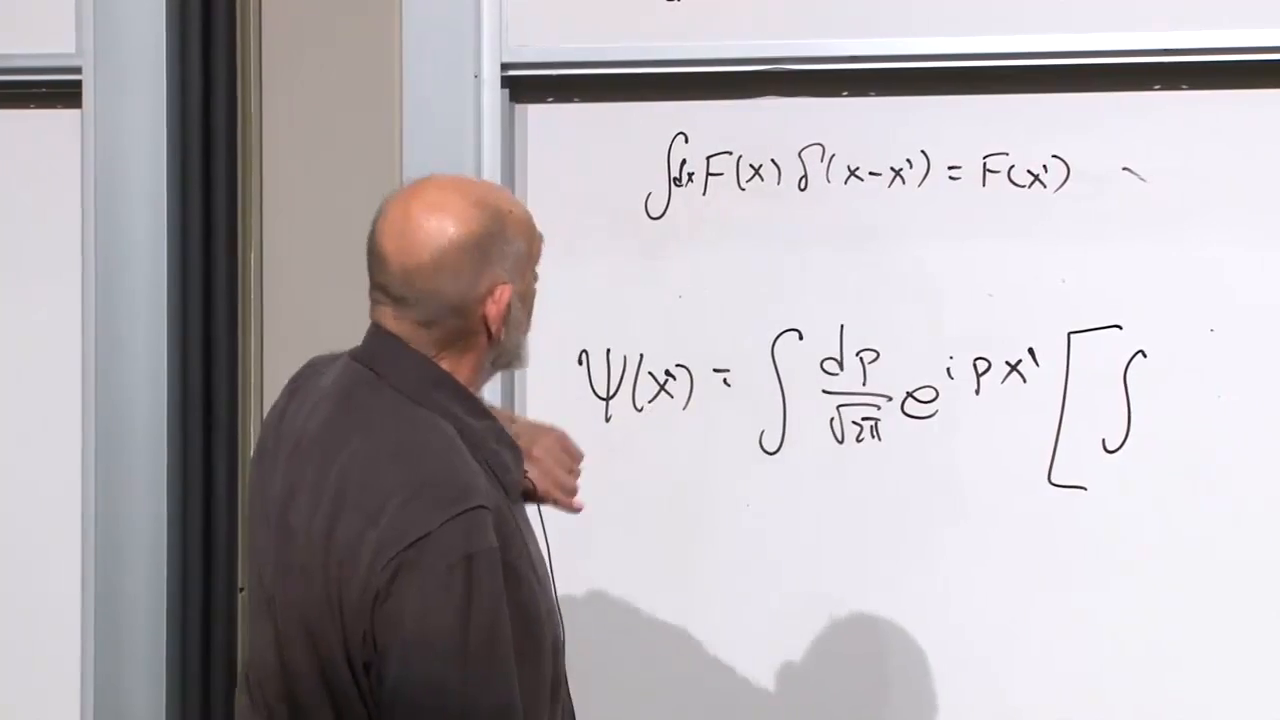
\includegraphics[width=0.88\textwidth]{lecture_09_figure_02.png}
\caption{對稱的傅立葉變換對：將函數分解為平面波，再由逆變換求回各模式的振幅。}
\lectureframe{00:14:35}
\end{figure}

\begin{classroomqa}
\audiencequestion{\(\psi(x)\)和\(\widetilde{\psi}(p)\)都預設為複數嗎？}
\lecturerresponse{一般而言，是的。某些特殊函數可能恰好是實數；此時其傅立葉係數會滿足額外的共軛關係。但量子振幅本來就自然地取複數，這裡不加上實數限制。}
\end{classroomqa}

\begin{classroomqa}
\audiencequestion{為什麼採用對稱因子\(1/\sqrt{2\pi}\)，而不把全部的\(2\pi\)都放在其中一個變換裡？}
\lecturerresponse{兩種慣例都一致。採用對稱的形式，正變換和逆變換便只差在指數的正負號。只要所有相關的歸一化也一致地調整，物理預測就不受慣例影響。}
\end{classroomqa}

\(x\)與\(p\)之間的互易關係已經顯現出來。一個函數可以透過對另一個變數積分來表示。目前這還只是傅立葉分析；很快，這一對變數就會成為位置和動量。

\section{狄拉克 {\proseunicodefont δ} 函數的運算定義}

直觀來說，{\proseunicodefont δ} 函數是寬度趨近於零、高度發散但面積為一的尖峰。這種圖像很有用，但運算上的定義更可靠。對每一個合適的測試函數\(f\)，都有
\begin{equation}
\int_{-\infty}^{\infty}
dx\,\delta(x-x')f(x)
=f(x').
\label{eq:l9-delta-sampling}
\end{equation}
以下三條常見規則表達的是同一個概念：
\begin{align}
f(x)\delta(x-x')
&=
f(x')\delta(x-x'),
\label{eq:l9-delta-multiplication}\\
\int_{-\infty}^{\infty}dx\,\delta(x-x')
&=1,
\label{eq:l9-delta-area}\\
\int_{-\infty}^{\infty}dx\,\delta(x-x')f(x)
&=f(x').
\end{align}
第一條規則成立，是因為 {\proseunicodefont δ} 函數只有在\(x=x'\)處才有支撐。在第二條規則中，平移尖峰只會改變其位置，不會改變其面積。將這兩條規則合併，就得到第三條。

\begin{figure}[htbp]
\centering
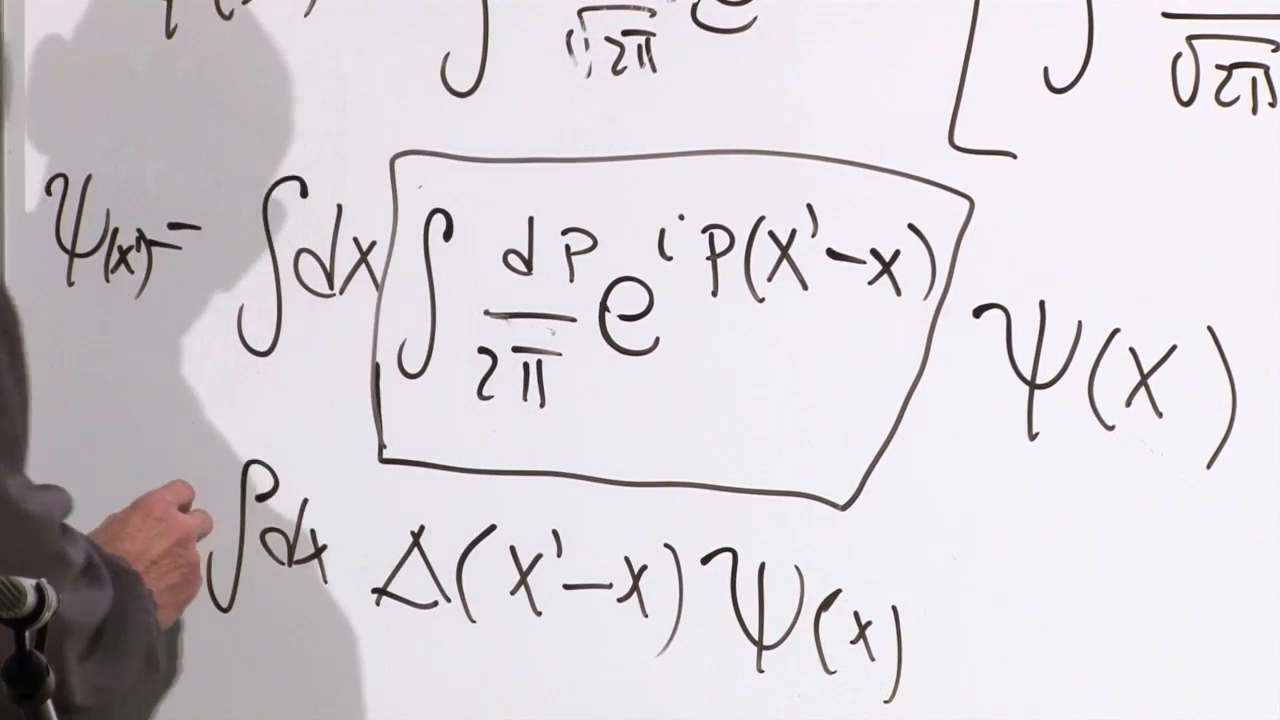
\includegraphics[width=0.88\textwidth]{lecture_09_figure_03.png}
\caption{狄拉克 {\proseunicodefont δ} 函數的抽樣性質：它對每個合適函數的作用都由此刻畫。}
\lectureframe{00:19:45}
\end{figure}

\begin{classroomqa}
\audiencequestion{為什麼可以把\(f(x')\)提出\(x\)積分之外？}
\lecturerresponse{積分變數是\(x\)。進行這個積分時，標記\(x'\)固定不變，因此\(f(x')\)相對於\(x\)是常數。剩下的 {\proseunicodefont δ} 積分面積為一。}
\end{classroomqa}

{\proseunicodefont δ} 函數不是一般的逐點函數。尤其是，將它平方會得到比原本的 {\proseunicodefont δ} 函數更奇異的物件。它較妥當的意義是分布：方程式~\eqref{eq:l9-delta-sampling}說明它在積分中的作用。

\subsection{{\proseunicodefont δ} 函數的傅立葉表示}

將方程式~\eqref{eq:l9-fourier-inverse}代入方程式~\eqref{eq:l9-fourier-forward}，並把左側的自變數改記為\(x'\)：
\begin{align}
\psi(x')
&=
\int\frac{dp}{\sqrt{2\pi}}\,
e^{ipx'}
\left[
\int\frac{dx}{\sqrt{2\pi}}\,
\psi(x)e^{-ipx}
\right] \notag\\
&=
\int dx
\left[
\int\frac{dp}{2\pi}
e^{ip(x'-x)}
\right]\psi(x).
\label{eq:l9-fourier-composition}
\end{align}
方括號中的表示式對每個合適的\(\psi\)都必須重現\(\psi(x')\)。與 {\proseunicodefont δ} 函數的定義性作用比較，可得
\begin{equation}
\boxed{
\int_{-\infty}^{\infty}
\frac{dp}{2\pi}\,
e^{ip(x'-x)}
=\delta(x'-x)
}.
\label{eq:l9-delta-fourier-x}
\end{equation}

\begin{figure}[htbp]
\centering
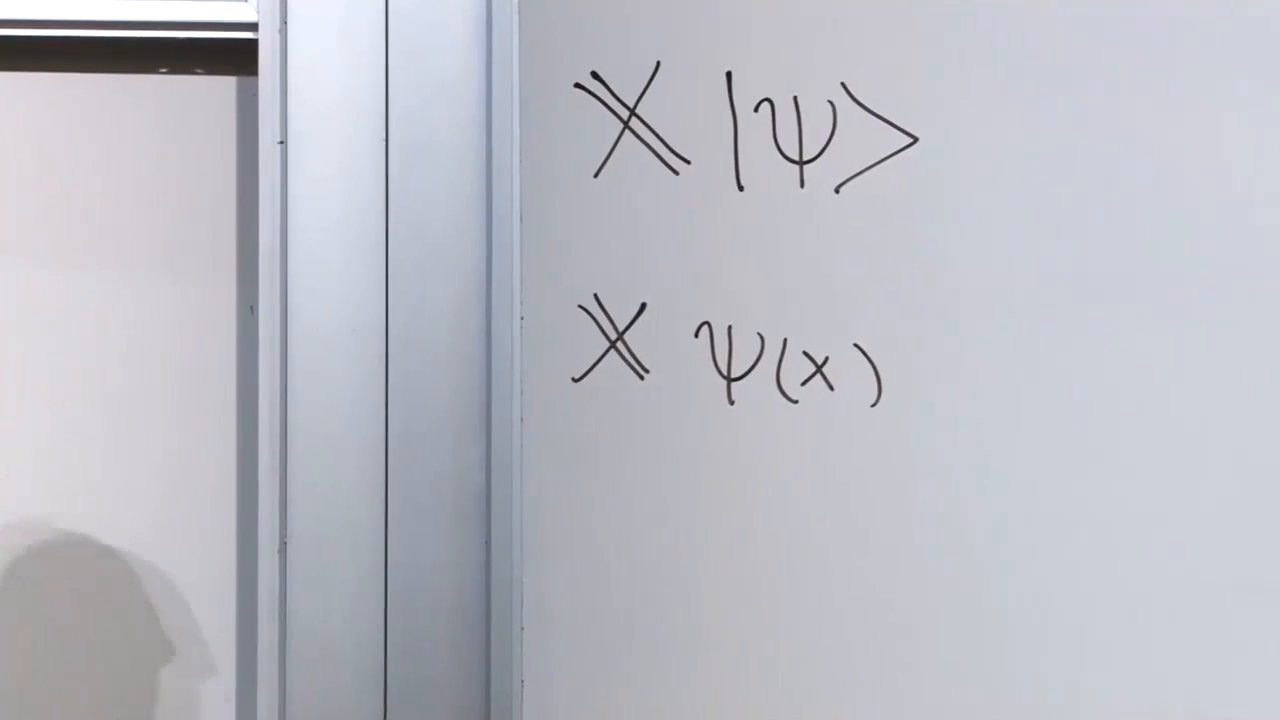
\includegraphics[width=0.88\textwidth]{lecture_09_figure_04.png}
\caption{在兩個變換的複合運算中分離出傅立葉核，再依其抽樣作用辨認出它就是狄拉克 {\proseunicodefont δ} 函數。}
\lectureframe{00:26:23}
\end{figure}

交換這一對互易變數的名稱，就得到相應的恆等式
\begin{equation}
\boxed{
\int_{-\infty}^{\infty}
\frac{dx}{2\pi}\,
e^{ix(p-p')}
=\delta(p-p')
}.
\label{eq:l9-delta-fourier-p}
\end{equation}
因此，{\proseunicodefont δ} 函數可以表示為平面波的連續疊加。

\begin{classroomqa}
\audiencequestion{指數有時寫成\(x'-x\)，有時寫成\(x-x'\)。正負號改變會影響結果嗎？}
\lecturerresponse{不會。{\proseunicodefont δ} 函數是偶函數：\(\delta(u)=\delta(-u)\)。因此，將差值的正負號反轉，不會改變最後得到的分布。中間的指數會變成其複共軛，但積分後的核仍是同一個 {\proseunicodefont δ} 函數。}
\end{classroomqa}

這些推導省略了一項關於收斂性的限定。振盪積分是分布，不是絕對收斂的一般積分；交換積分次序必須謹慎。有限的週期區間能提供乾淨的正則化方式：先使用離散傅立葉模式與克羅內克正交關係，再讓區間無限擴大。上面的連續恆等式就是這個極限。

\section{直線上的粒子}

在經典力學中，相空間中的一個點就能指定狀態：
\begin{equation}
(x,p).
\end{equation}
量子力學首先要問的則是：用什麼正交歸一基底來定義狀態空間？對每個實數位置\(x\)，引入廣義本徵態\(\ket{x}\)。一般狀態可以展開為
\begin{equation}
\ket{\Psi}
=
\int_{-\infty}^{\infty}
dx\,\psi(x)\ket{x},
\qquad
\psi(x)=\braket{x}{\Psi}.
\label{eq:l9-position-expansion}
\end{equation}

\begin{figure}[htbp]
\centering
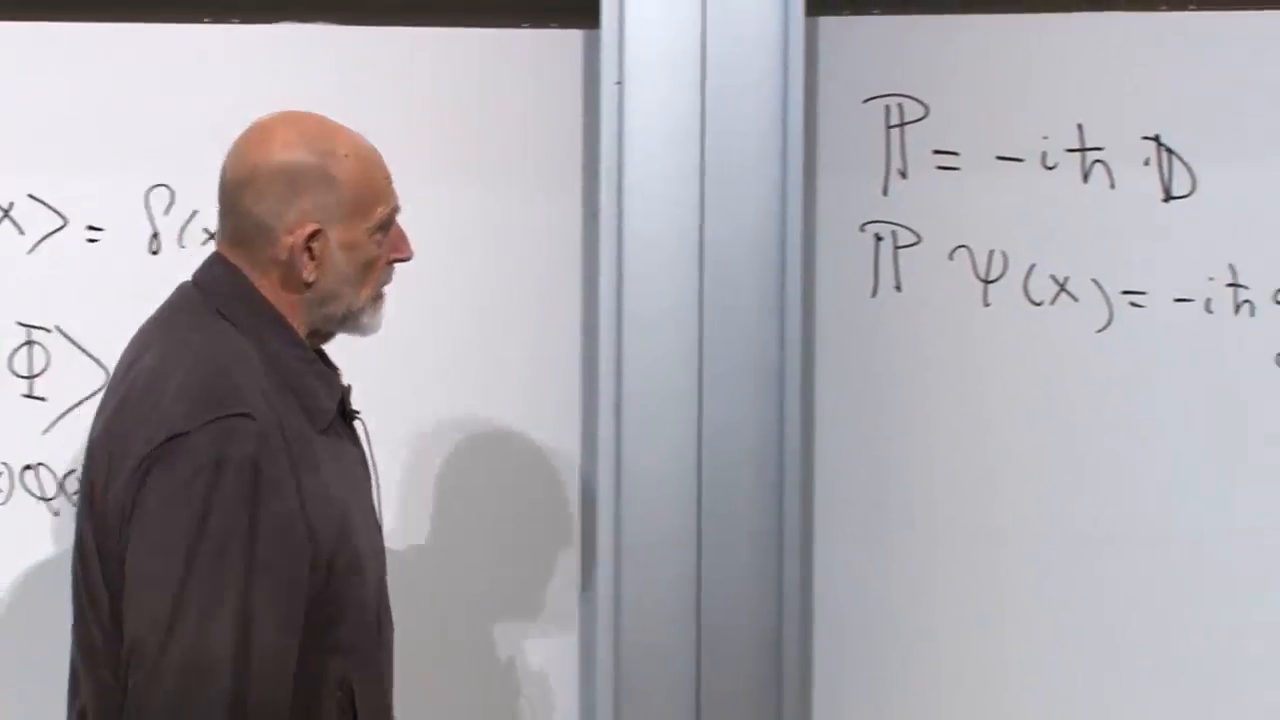
\includegraphics[width=0.88\textwidth]{lecture_09_figure_05.png}
\caption{一般狀態在連續位置基底中的展開；投影到\(\ket{x}\)上即可求回其係數。}
\lectureframe{00:35:30}
\end{figure}

玻恩規則給出的機率密度為
\begin{equation}
\rho(x)=|\psi(x)|^2.
\end{equation}
有限區間內的機率為
\begin{equation}
P(a<x<b)=\int_a^b|\psi(x)|^2\,dx,
\end{equation}
而歸一化的物理狀態滿足
\begin{equation}
\int_{-\infty}^{\infty}|\psi(x)|^2\,dx=1.
\label{eq:l9-position-normalization}
\end{equation}
連續基底的正交關係表示為
\begin{equation}
\braket{x'}{x}=\delta(x-x').
\label{eq:l9-position-delta}
\end{equation}
任意兩個狀態的內積則為
\begin{equation}
\braket{\Psi}{\Phi}
=
\int_{-\infty}^{\infty}
dx\,\psi^*(x)\phi(x).
\label{eq:l9-position-inner-product}
\end{equation}

\begin{figure}[htbp]
\centering
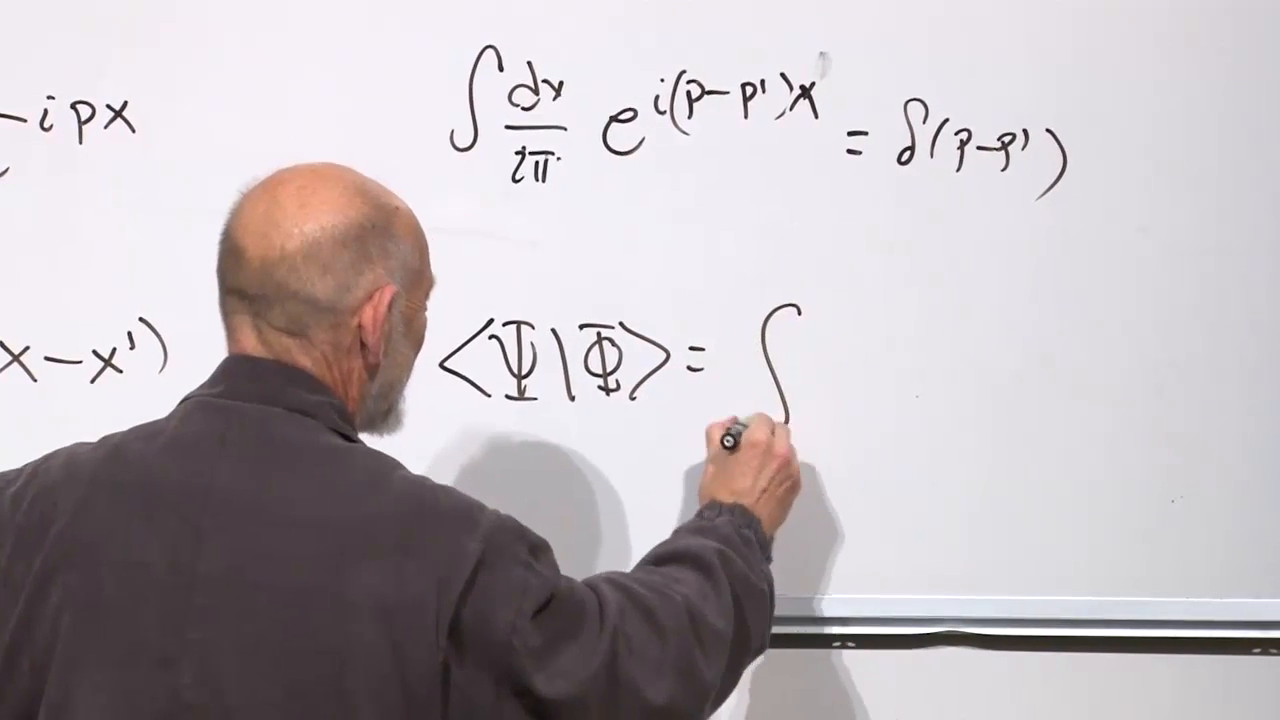
\includegraphics[width=0.88\textwidth]{lecture_09_figure_06.png}
\caption{連續基底的歸一化關係，以及以位置表象表示的波函數內積。}
\lectureframe{00:41:20}
\end{figure}

\begin{classroomqa}
\audiencequestion{為什麼只用位置就足夠？加入動量或幾乎任何其他變數，會不會是多餘的？}
\lecturerresponse{對一維中的單一粒子而言，完整的函數\(\psi(x)\)就能指定狀態，因此再指定\(p\)的確定值會提供過多資訊。動量提供的是另一組完備基底，而不是附加在每個\(\ket{x}\)上的標記。在更多維度中，可以混合彼此相容的資訊：例如，\(X\)與\(P_y\)對易，因此可共同標記一組基底。限制在於成對的不對易量，而非符號的數目。}
\end{classroomqa}

\begin{classroomqa}
\audiencequestion{動量也能提供一組完備基底，並透過位置表象展開嗎？}
\lecturerresponse{可以。動量基底是完備的，其係數透過傅立葉變換與位置表象的係數相互關聯。這個關係正是本講的核心構想。}
\end{classroomqa}

\section{位置表象中的位置算符}

抽象算符作用在狀態向量上。選定基底後，同一個作用就成為對波函數的具體運算。在位置表象中，位置算符\(X\)以乘法方式作用：
\begin{equation}
(X\psi)(x)=x\psi(x).
\label{eq:l9-position-operator}
\end{equation}

定域於\(x_0\)的狀態，以廣義波函數\(\delta(x-x_0)\)表示。讓\(X\)作用其上，可得
\begin{align}
X\delta(x-x_0)
&=
x\delta(x-x_0) \notag\\
&=
x_0\delta(x-x_0),
\label{eq:l9-position-eigenfunction}
\end{align}
這裡用到了方程式~\eqref{eq:l9-delta-multiplication}。因此，\(\delta(x-x_0)\)是\(X\)的本徵函數，其本徵值為\(x_0\)。

\begin{figure}[htbp]
\centering
\includegraphics[width=0.88\textwidth]{lecture_09_figure_07.png}
\caption{乘上\(x\)後，{\proseunicodefont δ} 定域態變成自身乘以\(x_0\)，因此可知它是位置本徵函數。}
\lectureframe{00:45:50}
\end{figure}

\(\ket{x_0}\)及其 {\proseunicodefont δ} 函數表示，都不符合一般平方可積意義下的單位歸一化，而是採用 {\proseunicodefont δ} 歸一化。物理上的局域態是有限寬度的波包；精確本徵態則作為廣義基底向量使用。

\section{動量本徵函數}

上一講發現，微分算符是反厄米的；乘上\(-i\)後，則成為厄米算符。恢復單位後，定義
\begin{equation}
P=-i\hbar\frac{d}{dx},
\qquad
(P\psi)(x)
=
-i\hbar\frac{d\psi}{dx}.
\label{eq:l9-momentum-operator}
\end{equation}
在適當的定義域上，這是合法的可觀測量。接下來會檢驗它是否就是物理動量，檢驗依據包括其譜、波長及其在動力學中的作用。

對動量本徵值\(p\)，求解
\begin{equation}
P\psi_p=p\psi_p,
\end{equation}
亦即
\begin{equation}
-i\hbar\frac{d\psi_p}{dx}=p\psi_p.
\end{equation}
解為
\begin{equation}
\psi_p(x)=A e^{ipx/\hbar}.
\label{eq:l9-momentum-eigenfunction}
\end{equation}

\begin{figure}[htbp]
\centering
\includegraphics[width=0.88\textwidth]{lecture_09_figure_08.png}
\caption{確定動量狀態在位置空間中的表示是一個平面波\(e^{ipx/\hbar}\)。}
\lectureframe{00:51:45}
\end{figure}

波長\(\lambda\)是使相位增加\(2\pi\)的位移：
\begin{equation}
\frac{p\lambda}{\hbar}=2\pi,
\qquad
\lambda=\frac{2\pi\hbar}{p}.
\label{eq:l9-de-broglie}
\end{equation}
因此，動量越大，波長越短。

{\proseunicodefont δ} 歸一化決定了常數：
\begin{equation}
\psi_p(x)
=
\frac{1}{\sqrt{2\pi\hbar}}e^{ipx/\hbar}.
\label{eq:l9-normalized-momentum-eigenfunction}
\end{equation}
確實，
\begin{align}
\braket{p'}{p}
&=
\int_{-\infty}^{\infty}
dx\,
\psi_{p'}^*(x)\psi_p(x) \notag\\
&=
\int_{-\infty}^{\infty}
\frac{dx}{2\pi\hbar}
e^{i(p-p')x/\hbar} \notag\\
&=
\delta(p-p').
\label{eq:l9-momentum-normalization}
\end{align}
選用\(\hbar=1\)的單位後，這些公式成為
\begin{equation}
\psi_p(x)=\frac{1}{\sqrt{2\pi}}e^{ipx},
\qquad
\int\frac{dx}{2\pi}e^{i(p-p')x}
=\delta(p-p').
\end{equation}

\begin{classroomqa}
\audiencequestion{當振盪積分在一般意義下並不收斂時，為什麼能說它在\(p\neq p'\)時等於零？}
\lecturerresponse{本講採用一種受控的簡化做法。把系統置於有限的週期區間中，允許的動量便形成離散集合，指數函數也具有一般意義下的正交性，而且所有歸一化都有限。完成這項計算後，才讓區間趨向無窮大，將克羅內克 {\proseunicodefont δ} 轉為狄拉克 {\proseunicodefont δ}。}
\end{classroomqa}

\begin{classroomqa}
\audiencequestion{{\proseunicodefont δ} 函數的傅立葉變換推導也有相同的收斂問題嗎？}
\lecturerresponse{有。基於相同原因，那裡交換積分次序的步驟也是形式上的。有限盒子的推導或分布的數學語言，可以補上省略的嚴謹論證。由於經過正則化的計算確實有前述連續極限，這種簡化做法是可接受的。}
\end{classroomqa}

\section{動量表象}

有兩個物件不能混為一談。方程式~\eqref{eq:l9-normalized-momentum-eigenfunction}中的函數\(\psi_p(x)\)，是特定本徵態\(\ket{p}\)在位置空間中的表示。相較之下，任意狀態\(\ket{\Psi}\)的動量空間波函數為
\begin{equation}
\widetilde{\psi}(p)=\braket{p}{\Psi}.
\label{eq:l9-momentum-wavefunction}
\end{equation}
代入\(\bra{p}\)和\(\ket{\Psi}\)在位置空間中的波函數：
\begin{align}
\widetilde{\psi}(p)
&=
\int_{-\infty}^{\infty}
dx\,
\braket{p}{x}\braket{x}{\Psi} \notag\\
&=
\int_{-\infty}^{\infty}
\frac{dx}{\sqrt{2\pi\hbar}}\,
e^{-ipx/\hbar}\psi(x).
\label{eq:l9-position-to-momentum}
\end{align}
這正是傅立葉變換。反過來，
\begin{equation}
\psi(x)
=
\int_{-\infty}^{\infty}
\frac{dp}{\sqrt{2\pi\hbar}}\,
\widetilde{\psi}(p)e^{ipx/\hbar}.
\label{eq:l9-momentum-to-position}
\end{equation}

\begin{figure}[htbp]
\centering
\includegraphics[width=0.88\textwidth]{lecture_09_figure_09.png}
\caption{投影到\(\ket{p}\)上，便將位置空間波函數轉換為其傅立葉變換\(\widetilde{\psi}(p)\)。}
\lectureframe{01:05:50}
\end{figure}

測量動量\(p\)的機率密度為
\begin{equation}
\widetilde{\rho}(p)
=
|\widetilde{\psi}(p)|^2,
\qquad
\int_{-\infty}^{\infty}
|\widetilde{\psi}(p)|^2\,dp=1.
\end{equation}
因此，單一位置空間波函數已包含足夠資訊，可以預測位置和動量測量的結果。若要得到動量機率，就對\(\psi(x)\)作傅立葉變換，再取結果的絕對值平方。

在動量表象中，兩個算符的角色互換：
\begin{equation}
(P\widetilde{\psi})(p)
=
p\widetilde{\psi}(p),
\qquad
(X\widetilde{\psi})(p)
=
i\hbar\frac{d\widetilde{\psi}}{dp}.
\label{eq:l9-operators-in-p}
\end{equation}
與\(P=-i\hbar\,d/dx\)的符號不同，是因為傅立葉變換對中的指數符號相反。

\begin{classroomqa}
\audiencequestion{時間是否也像位置與動量那樣，是與能量共軛的算符？}
\lecturerresponse{通常將時間視為標記狀態演化的外部參數，而非系統希爾伯特空間上的通用自伴算符。物理時鐘確實有可觀測的讀數，而提高時鐘的時間解析度會帶來能量上的影響；但時間與能量的關係比位置與動量這一對更需要謹慎處理，本講不會深入探討。}
\end{classroomqa}

\begin{classroomqa}
\audiencequestion{還有哪些共軛變數對？}
\lecturerresponse{角度與相應的角動量是重要例子，但由於角度具有週期性，還需考慮整體上的限制。在場論中，場與其正則動量互為共軛。溫度與壓力是熱力學變數，不是正則量子共軛對。一般原理由正則變數及其對易關係決定，不是任意一對可觀測量都符合。}
\end{classroomqa}

\begin{classroomqa}
\audiencequestion{在離散理論中，算符作用於右矢，而波函數只是列出係數。到了連續理論，情況改變了嗎？}
\lecturerresponse{沒有改變。波函數是抽象右矢在選定基底中的座標列。作用在有限維列向量上的矩陣，與作用在函數上的微分或積分算符，都是同一個抽象運算的具體表示。連續標記改變的是記號，而非邏輯。}
\end{classroomqa}

\subsection{傅立葉變換所揭示的不確定性}

動量確定的狀態完全離域：
\begin{equation}
|\psi_p(x)|^2=\text{constant}.
\end{equation}
其動量是確定的，但位置均勻分布於整條直線上。更一般地說，一對傅立葉變換不可能同時都很窄。將\(\widetilde{\psi}(p)\)集中在很小的動量範圍內，會迫使\(\psi(x)\)延伸到很大的區域；而要讓\(\psi(x)\)局域化，就需要涵蓋很廣的動量範圍。

本講尚未推導定量的不等式
\begin{equation}
\Delta X\,\Delta P\geq\frac{\hbar}{2}.
\end{equation}
此處要強調的是結構上的要點：不確定性原理已經蘊含在傅立葉變換的互易幾何中。這相當於連續情況下，在不相容的自旋基底之間變換。

\section{哈密頓量生成時間演化}

哈密頓量\(H\)是厄米算符，代表能量，並生成么正時間演化。含時Schr\"odinger方程為
\begin{equation}
i\hbar\frac{d}{dt}\ket{\Psi(t)}
=
H\ket{\Psi(t)}.
\label{eq:l9-abstract-schrodinger}
\end{equation}
在位置表象中，
\begin{equation}
i\hbar\frac{\partial\psi(x,t)}{\partial t}
=
H\psi(x,t),
\label{eq:l9-position-schrodinger}
\end{equation}
右側表示哈密頓量作用在函數上時，所採用的位置空間表示。

\subsection{刻意選取的簡單線性哈密頓量}

令
\begin{equation}
H=cP.
\label{eq:l9-linear-hamiltonian}
\end{equation}
這不是一般的非相對論自由粒子哈密頓量。選用它是因為每個步驟都能直接看清楚。

\begin{figure}[htbp]
\centering
\includegraphics[width=0.88\textwidth]{lecture_09_figure_10.png}
\caption{線性哈密頓量\(H=cP\)與Schr\"odinger方程；選用前者作為描述粒子演化的最簡單例子。}
\lectureframe{01:17:45}
\end{figure}

利用\(P=-i\hbar\,\partial_x\)，可得
\begin{align}
i\hbar\frac{\partial\psi}{\partial t}
&=
c\left(-i\hbar\frac{\partial}{\partial x}\right)\psi, \notag\\
\frac{\partial\psi}{\partial t}
&=
-c\frac{\partial\psi}{\partial x},
\end{align}
亦即
\begin{equation}
\frac{\partial\psi}{\partial t}
+c\frac{\partial\psi}{\partial x}=0.
\label{eq:l9-transport-equation}
\end{equation}

\begin{figure}[htbp]
\centering
\includegraphics[width=0.88\textwidth]{lecture_09_figure_11.png}
\caption{線性哈密頓量將Schr\"odinger方程化為一階輸運方程。}
\lectureframe{01:20:05}
\end{figure}

通解為
\begin{equation}
\psi(x,t)=f(x-ct),
\label{eq:l9-rigid-translation}
\end{equation}
其中\(f\)是任意可歸一化的初始分布。在\(t=0\)時，分布為\(f(x)\)。之後，整個分布的每個特徵都向右平移\(ct\)。複數波函數、它的實部和虛部，以及機率密度，都保持原有形狀：
\begin{equation}
|\psi(x,t)|^2=|f(x-ct)|^2.
\end{equation}
因此，
\begin{equation}
\expect{X}_t=\expect{X}_0+ct.
\end{equation}

符號\(c\)取來讓人聯想到光速。這個模型類似一種一維手性的無質量激發：每個允許的分量都以相同速率朝同一方向運動。它不是完整的光子理論。具有固定聲速的低能一維聲子，也提供了另一種類比。由於\(E=cp\)，允許\(p\)取正值或負值，也就會允許負能量；這再次表明它是刻意簡化的教學模型。

\begin{classroomqa}
\audiencequestion{如果把\(c\)換成某個自由粒子的速度，\(H=cP\)能描述該粒子嗎？}
\lecturerresponse{不能。\(H=cP\)中的係數固定，表示每個動量分量的速度都相同。非相對論粒子的速度是\(p/m\)，會隨動量而變。以\(v=p/m\)代入\(vP\)後，哈密頓量便不再是\(P\)的線性函數；這將導向二次型哈密頓量。}
\end{classroomqa}

\begin{classroomqa}
\audiencequestion{一般自由運動的電子，其波函數難道不應該只是整體平移而保持形狀嗎？}
\lecturerresponse{只有非常特殊的色散關係，才會讓任意分布都保持形狀平移。一般自由電子的波包包含許多動量分量，而它們的相位演化速率各不相同。波包中心會移動，但形狀通常會擴散。}
\end{classroomqa}

\subsection{與經典力學的比較}

對經典哈密頓量\(H=cp\)，哈密頓方程給出
\begin{equation}
\dot{x}=\frac{\partial H}{\partial p}=c,
\qquad
\dot{p}=-\frac{\partial H}{\partial x}=0.
\label{eq:l9-linear-hamilton-equations}
\end{equation}

\begin{figure}[htbp]
\centering
\includegraphics[width=0.88\textwidth]{lecture_09_figure_12.png}
\caption{\(H=cp\)的哈密頓方程：速度固定且向右，動量守恆。}
\lectureframe{01:25:20}
\end{figure}

量子機率分布及其期望值遵循同樣的基本運動。這種一致性初步具體說明，由經典哈密頓量構造的量子演化，應以適當的方式重現經典方程。

\section{非相對論自由粒子}

對於質量為\(m\)且不受力的一般粒子，經典動能為
\begin{equation}
H=\frac{p^2}{2m}.
\end{equation}
這個二次形式對\(p\)和\(-p\)一視同仁，因此向左和向右運動的粒子具有相同的正能量。量子化時，將\(p\)換成算符\(P\)：
\begin{equation}
H=\frac{P^2}{2m}.
\label{eq:l9-free-hamiltonian}
\end{equation}
將\(P=-i\hbar\,\partial_x\)代入Schr\"odinger方程：
\begin{align}
i\hbar\frac{\partial\psi}{\partial t}
&=
\frac{1}{2m}
\left(-i\hbar\frac{\partial}{\partial x}\right)^2
\psi \notag\\
&=
-\frac{\hbar^2}{2m}
\frac{\partial^2\psi}{\partial x^2}.
\label{eq:l9-free-schrodinger}
\end{align}

\begin{figure}[htbp]
\centering
\includegraphics[width=0.88\textwidth]{lecture_09_figure_13.png}
\caption{由\(H=P^2/(2m)\)和\(P=-i\hbar\,\partial_x\)得到的自由粒子Schr\"odinger方程。}
\lectureframe{01:33:50}
\end{figure}

動量為\(p\)的平面波分量，其能量為
\begin{equation}
E(p)=\frac{p^2}{2m}.
\end{equation}
與線性的\(E=cp\)情形不同，這個色散關係的斜率取決於\(p\)：
\begin{equation}
v_{\mathrm{group}}
=
\frac{dE}{dp}
=
\frac{p}{m}.
\end{equation}
因此，局域波包中不同動量分量的群速度各不相同。它們的相對相位會改變，各分量逐漸分離，波包因而擴散。關鍵差異在於，\(H=cP\)會讓任何形狀都保持不變地平移；\(H=P^2/(2m)\)則會造成自由粒子的色散運動。

\section{本講確立的內容}

這段數學討論並非與物理脫節。平面波和狄拉克 {\proseunicodefont δ} 函數建立了連續基底的架構。位置算符以乘法方式作用，動量算符以微分方式作用，而動量本徵態是平面波。將任意狀態投影到這些本徵態上，便得到其位置波函數的傅立葉變換。因此，位置和動量是描述同一狀態的兩種表象；它們的不確定性，正是傅立葉變換對熟悉的互易寬度關係。

接著，同一套表象架構將哈密頓量轉換為微分方程。動量的線性函數會造成形狀不變的平移；二次型動能則導出自由粒子的Schr\"odinger方程和色散。本課程已從測量的基礎進入運動力學，而核心語言始終不變：狀態、基底、厄米可觀測量、振幅和么正演化。
